%\setcounter{chapter}{31}

\chapter{Data Bias and Shift}
\label{chapter:bias_and_shift}
%\reviewcomment{Unfinished. To be added: connections to fairness and social bias, more examples.}

\section{Introduction}

The goal of learning is to acquire rules from past data that work well on future data. In the theory of machine learning, it is almost always assumed that the future is \textit{identically distributed} as the past. In reality, it is almost always the case that this is not true. Many of the failures of machine learning in industry and in society are due to this discrepancy between theory and practice.

What happens when a learned system is deployed on data that is unlike what it was trained on? In this chapter we will look just at what can go wrong, and in later chapters we will consider how we can mitigate these effects.

As a case study we will look at the paper ``Colorful Image Colorization''~\cite{zhang2016colorful}, which one of the authors of this book co-authored in 2016, so we don't feel too bad pointing out its flaws. In that paper, we trained a CNN to colorize black and white photos, and the results looked amazing (\fig{\ref{fig:bias_and_shift:CIC_teaser}}).
\begin{figure}[h!]
    \centerline{
    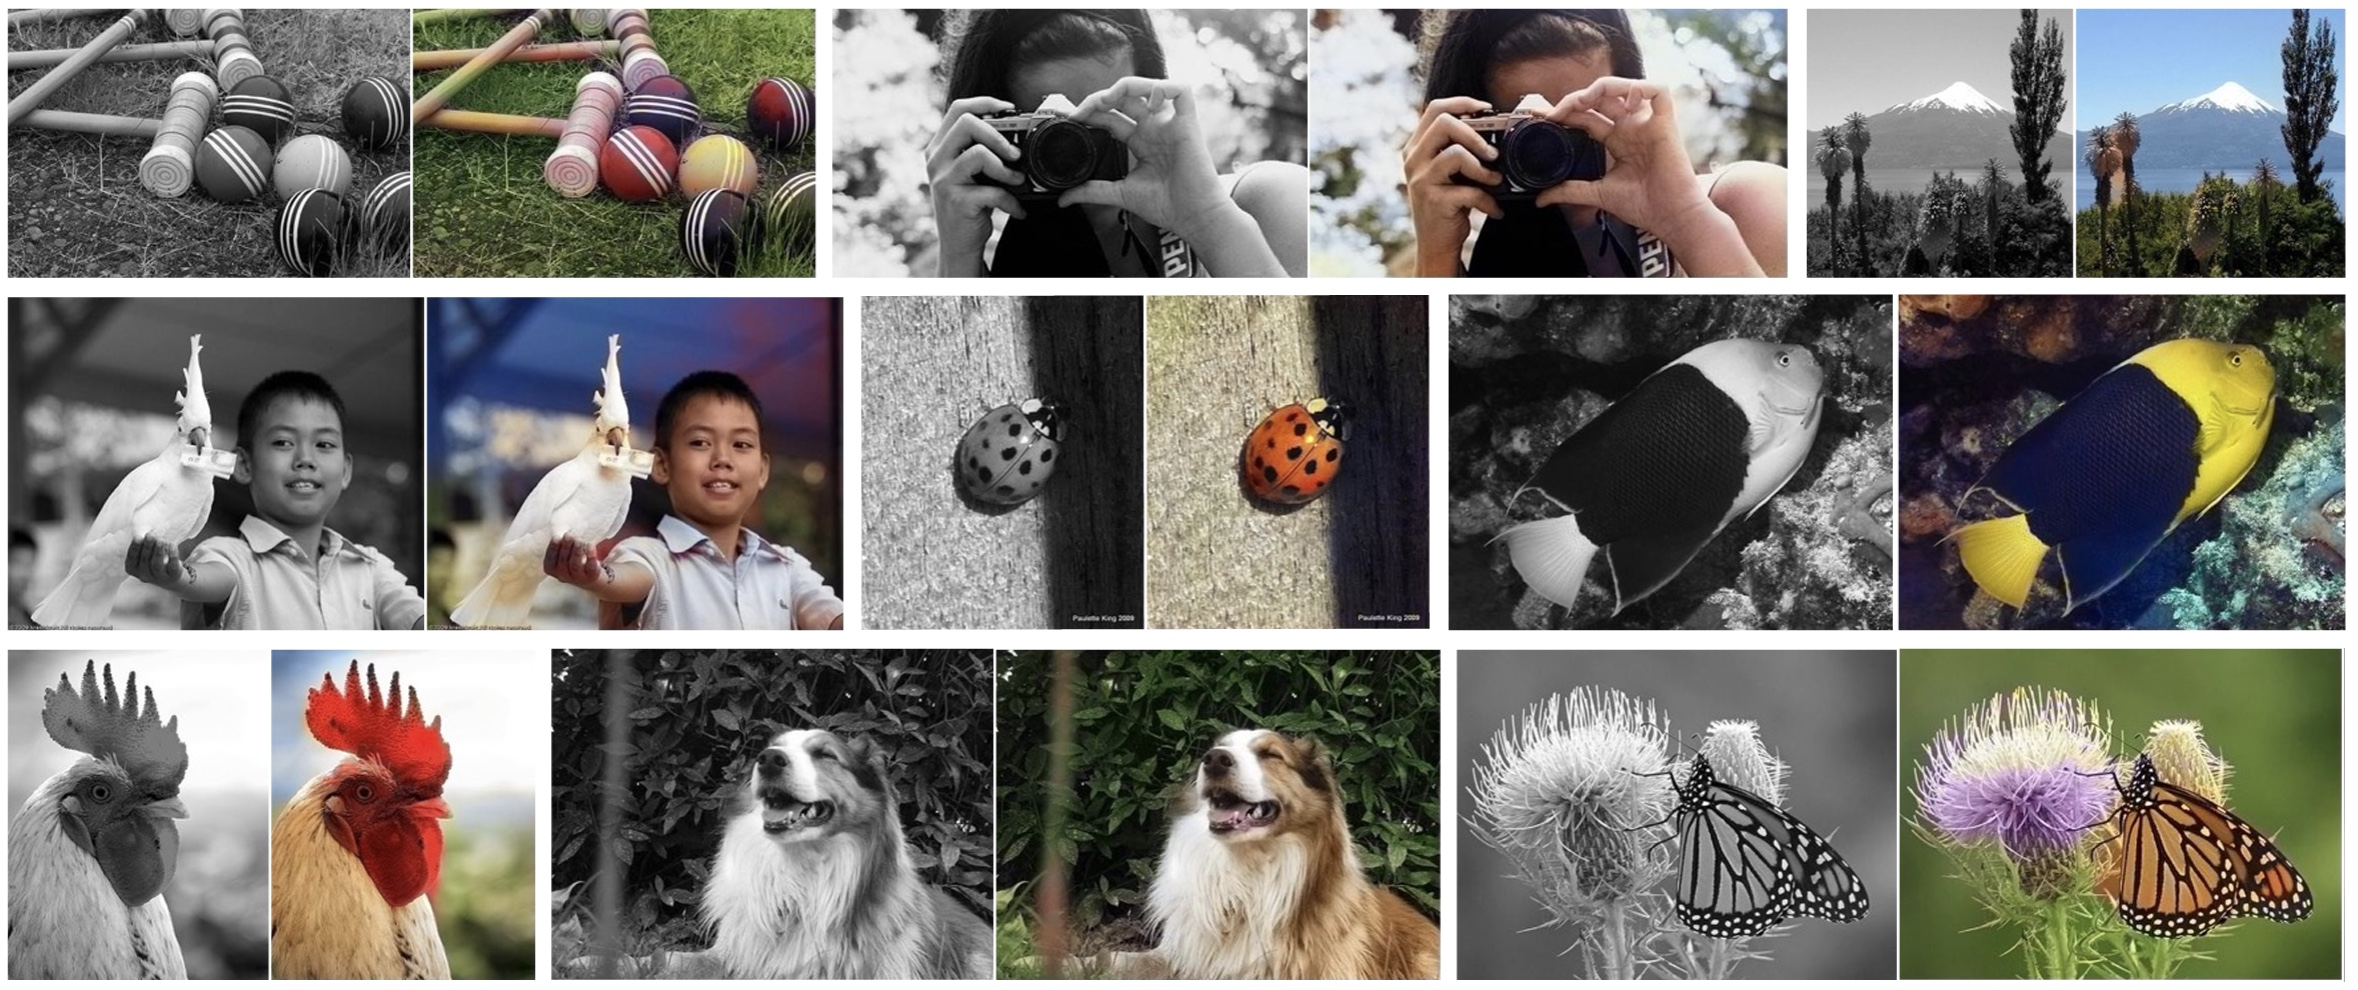
\includegraphics[width=1.0\linewidth]{./figures/bias_and_shift/CIC_teaser_v5.jpg}
    }
    \caption{Each pair of images shows the grayscale input image and, to its right, the output of the automatic colorization system. Source: \cite{zhang2016colorful}.}
    \label{fig:bias_and_shift:CIC_teaser}
\end{figure}

This was the teaser figure from our paper, showing sixteen examples of grayscale input images and the output of our system. Looks almost perfect, right? Well that's what people must have thought, because shortly after releasing our code, a user of the website Reddit\footnote{\texttt{http://www.reddit.com}} turned it into a bot called ColorizeBot\footnote{\texttt{http://www.reddit.com/user/pm\_me\_your\_bw\_pics}} that would colorize black and white photos posted on Reddit~\cite{colorizebot_blog}. In \fig{\ref{fig:bias_and_shift:colorizebot_examples}} are two of the more popular results.
\begin{figure}[h!]
    \centerline{
    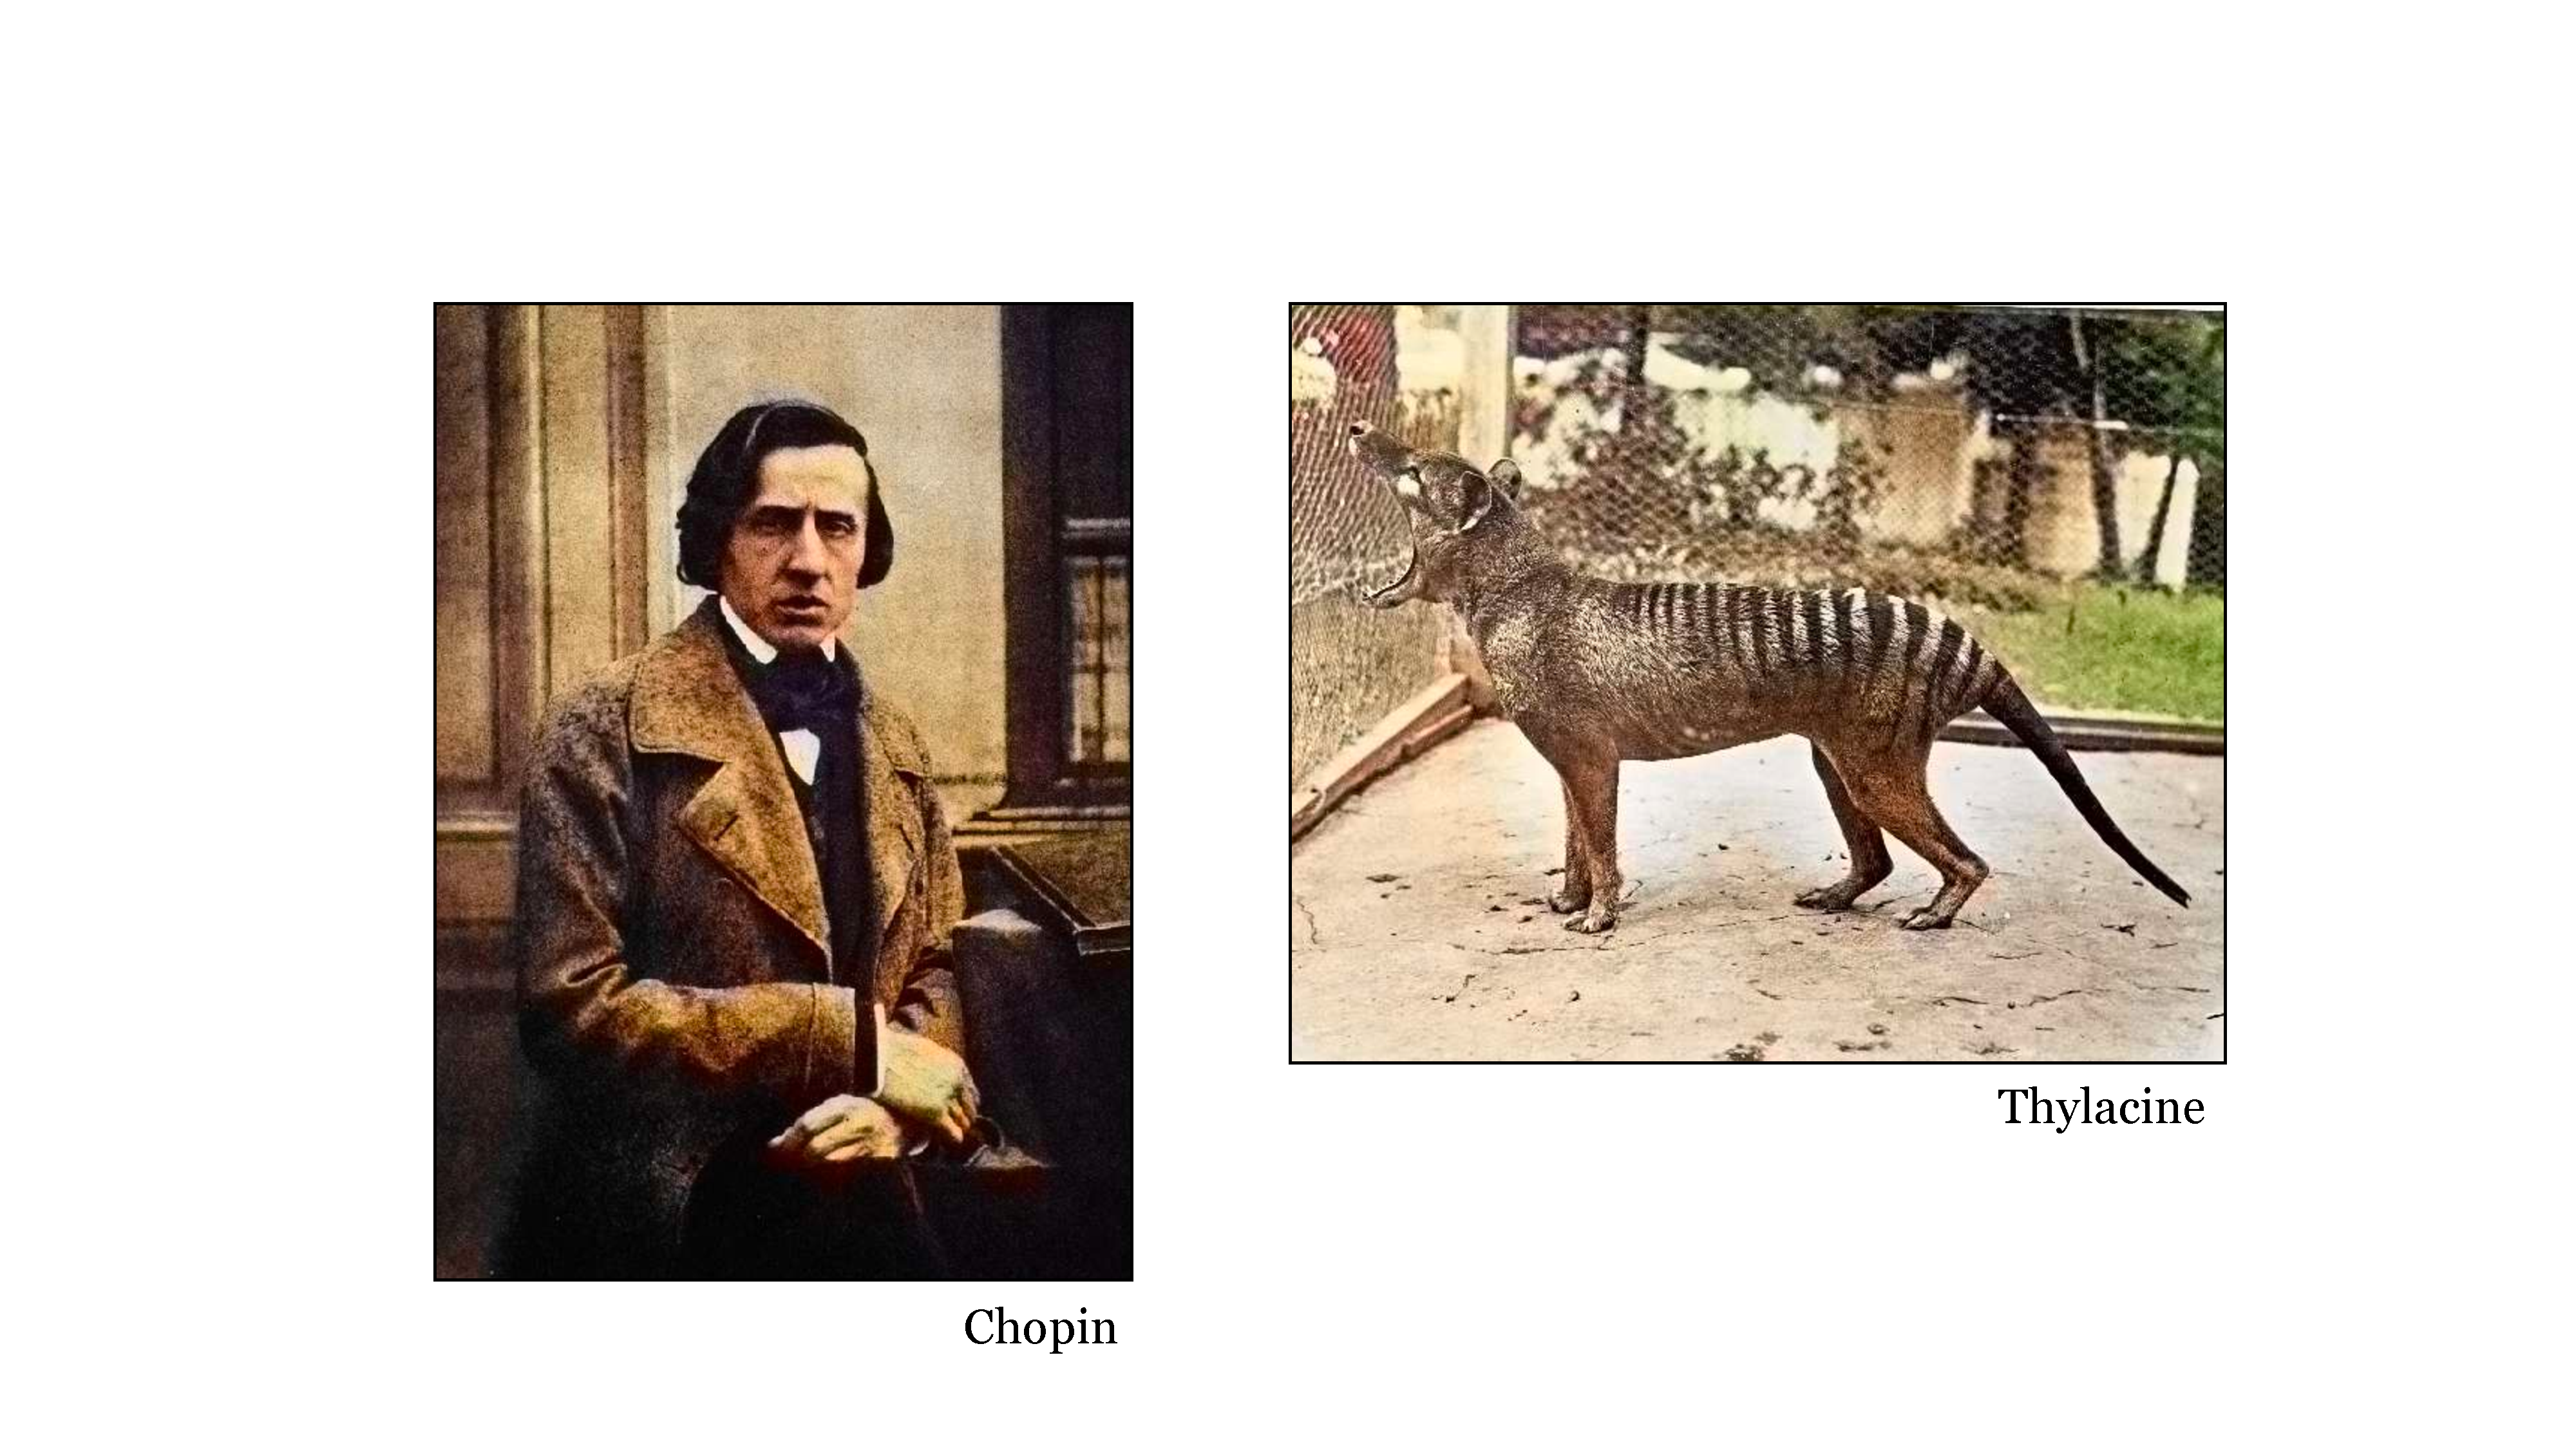
\includegraphics[width=0.7\linewidth]{./figures/bias_and_shift/colorizebot_examples.pdf}
    }
    \caption{Two results of Reddit's ColorizeBot~\cite{colorizebot_blog}. Original images are (left) Chopin, by Louis-Auguste Bisson, 1849, (right) and Benjamin the Thylacine, 1933. The bot ran the model from~\cite{zhang2016colorful} on the original black and white photos.}
    \label{fig:bias_and_shift:colorizebot_examples}
\end{figure}
%image urls: 
% \texttt{https://en.wikipedia.org/wiki/Fr\%C3\%A9d\%C3\%A9ric\_Chopin\#/media/File:Frederic\_Chopin\_photo.jpeg}
% \texttt{https://en.wikipedia.org/wiki/Thylacine\#/media/File:\%22Benjamin\%22.jpg}

The results were much worse than what we had shown in our paper. The bot turned most photos sepia-toned, and would frequently add ugly smudges of yellow and red. You might think, well the Reddit user must have implemented our method incorrectly, but that isn't it; to our knowledge, the code is correct. Why then, did it work so poorly?

The answer is data bias. We trained our colorization net on ImageNet. Reddit users tested it on famous historical photos, extinct animals, and old pictures of their family members. ImageNet is mostly photos of animals, along with a few other object categories. It does not contain many photos of scenes, and especially underrepresents humans, compared to how often people take photos of humans. In fact, a large percent of ImageNet photos are just dogs (around 12 percent). You can get an idea of the degree of the bias by looking at how our net colorizes the dogs in \fig{\ref{fig:bias_and_shift:dogs_with_tongues}}.
%\vspace{-0.4cm}
\begin{figure}[h!]
    \centerline{
    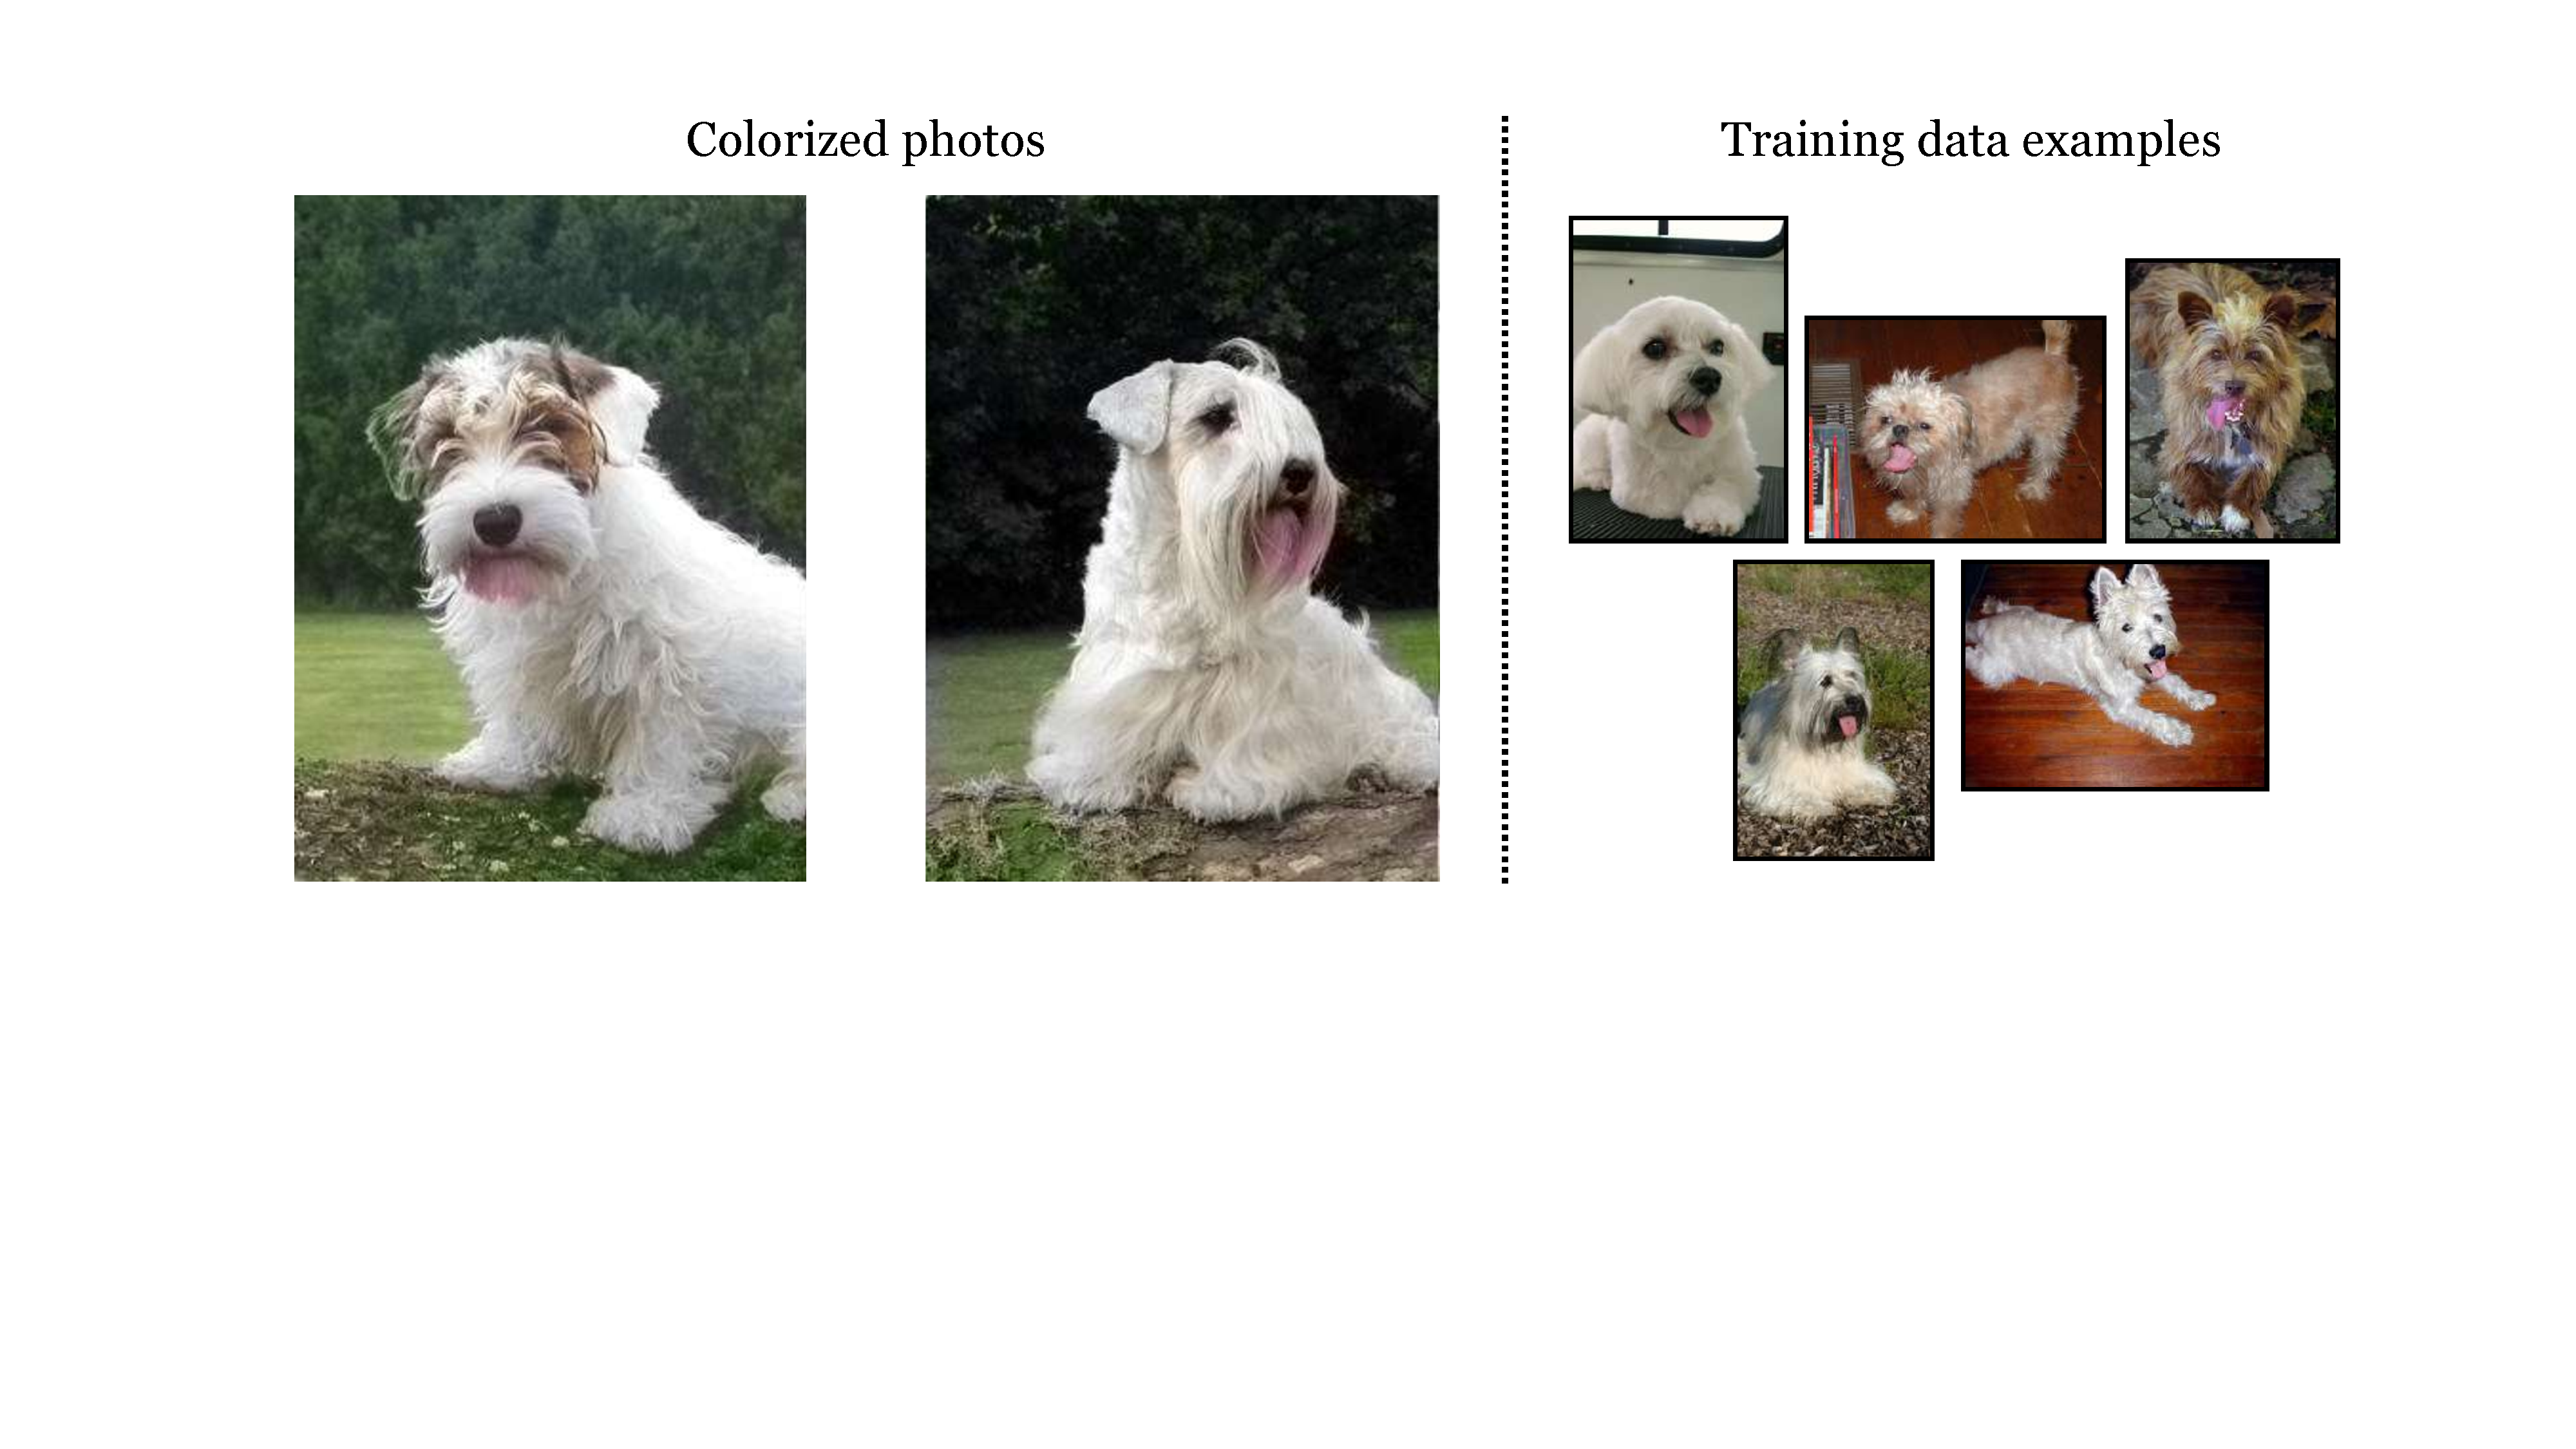
\includegraphics[width=0.9\linewidth]{./figures/bias_and_shift/dogs_with_tongues.pdf}
    }
    \caption{(left) Colorization results, using a model trained on ImageNet (example made by Richard Zhang; input black and white photos from ImageNet~\cite{russakovsky2015imagenet}). (right) Examples of dog images in ImageNet~\cite{russakovsky2015imagenet}. \reviewcomment{need permission?}}
    \label{fig:bias_and_shift:dogs_with_tongues}
\end{figure}

It adds a pinkish blob underneath their mouths! Why? Because not only is ImageNet full of dogs, it is full of dogs with their tongues out. So the net learned that it's a good strategy to put down a blob of pink whenever it detects a dog mouth, regardless of whether that mouth is open or closed.

Our net did not work well because the training data (ImageNet) was categorically different than the test data (photos uploaded on Reddit). This is true in terms of the content of the images but also in terms of the photographic style of the images. ImageNet is almost exclusively made up of photos taken with modern digital cameras. Reddit users were more interested in old photos taken with analog cameras, full of photographic grain and covered in dust and scratches.

\section{Out-of-Distribution Generalization}
\index{Out-of-distribution generalization}

To formalize what's going on, we will return to a simple regression problem, shown below (\fig{\ref{fig:bias_and_shift:regression_example}}).
\begin{figure}[h!]
    \centerline{
    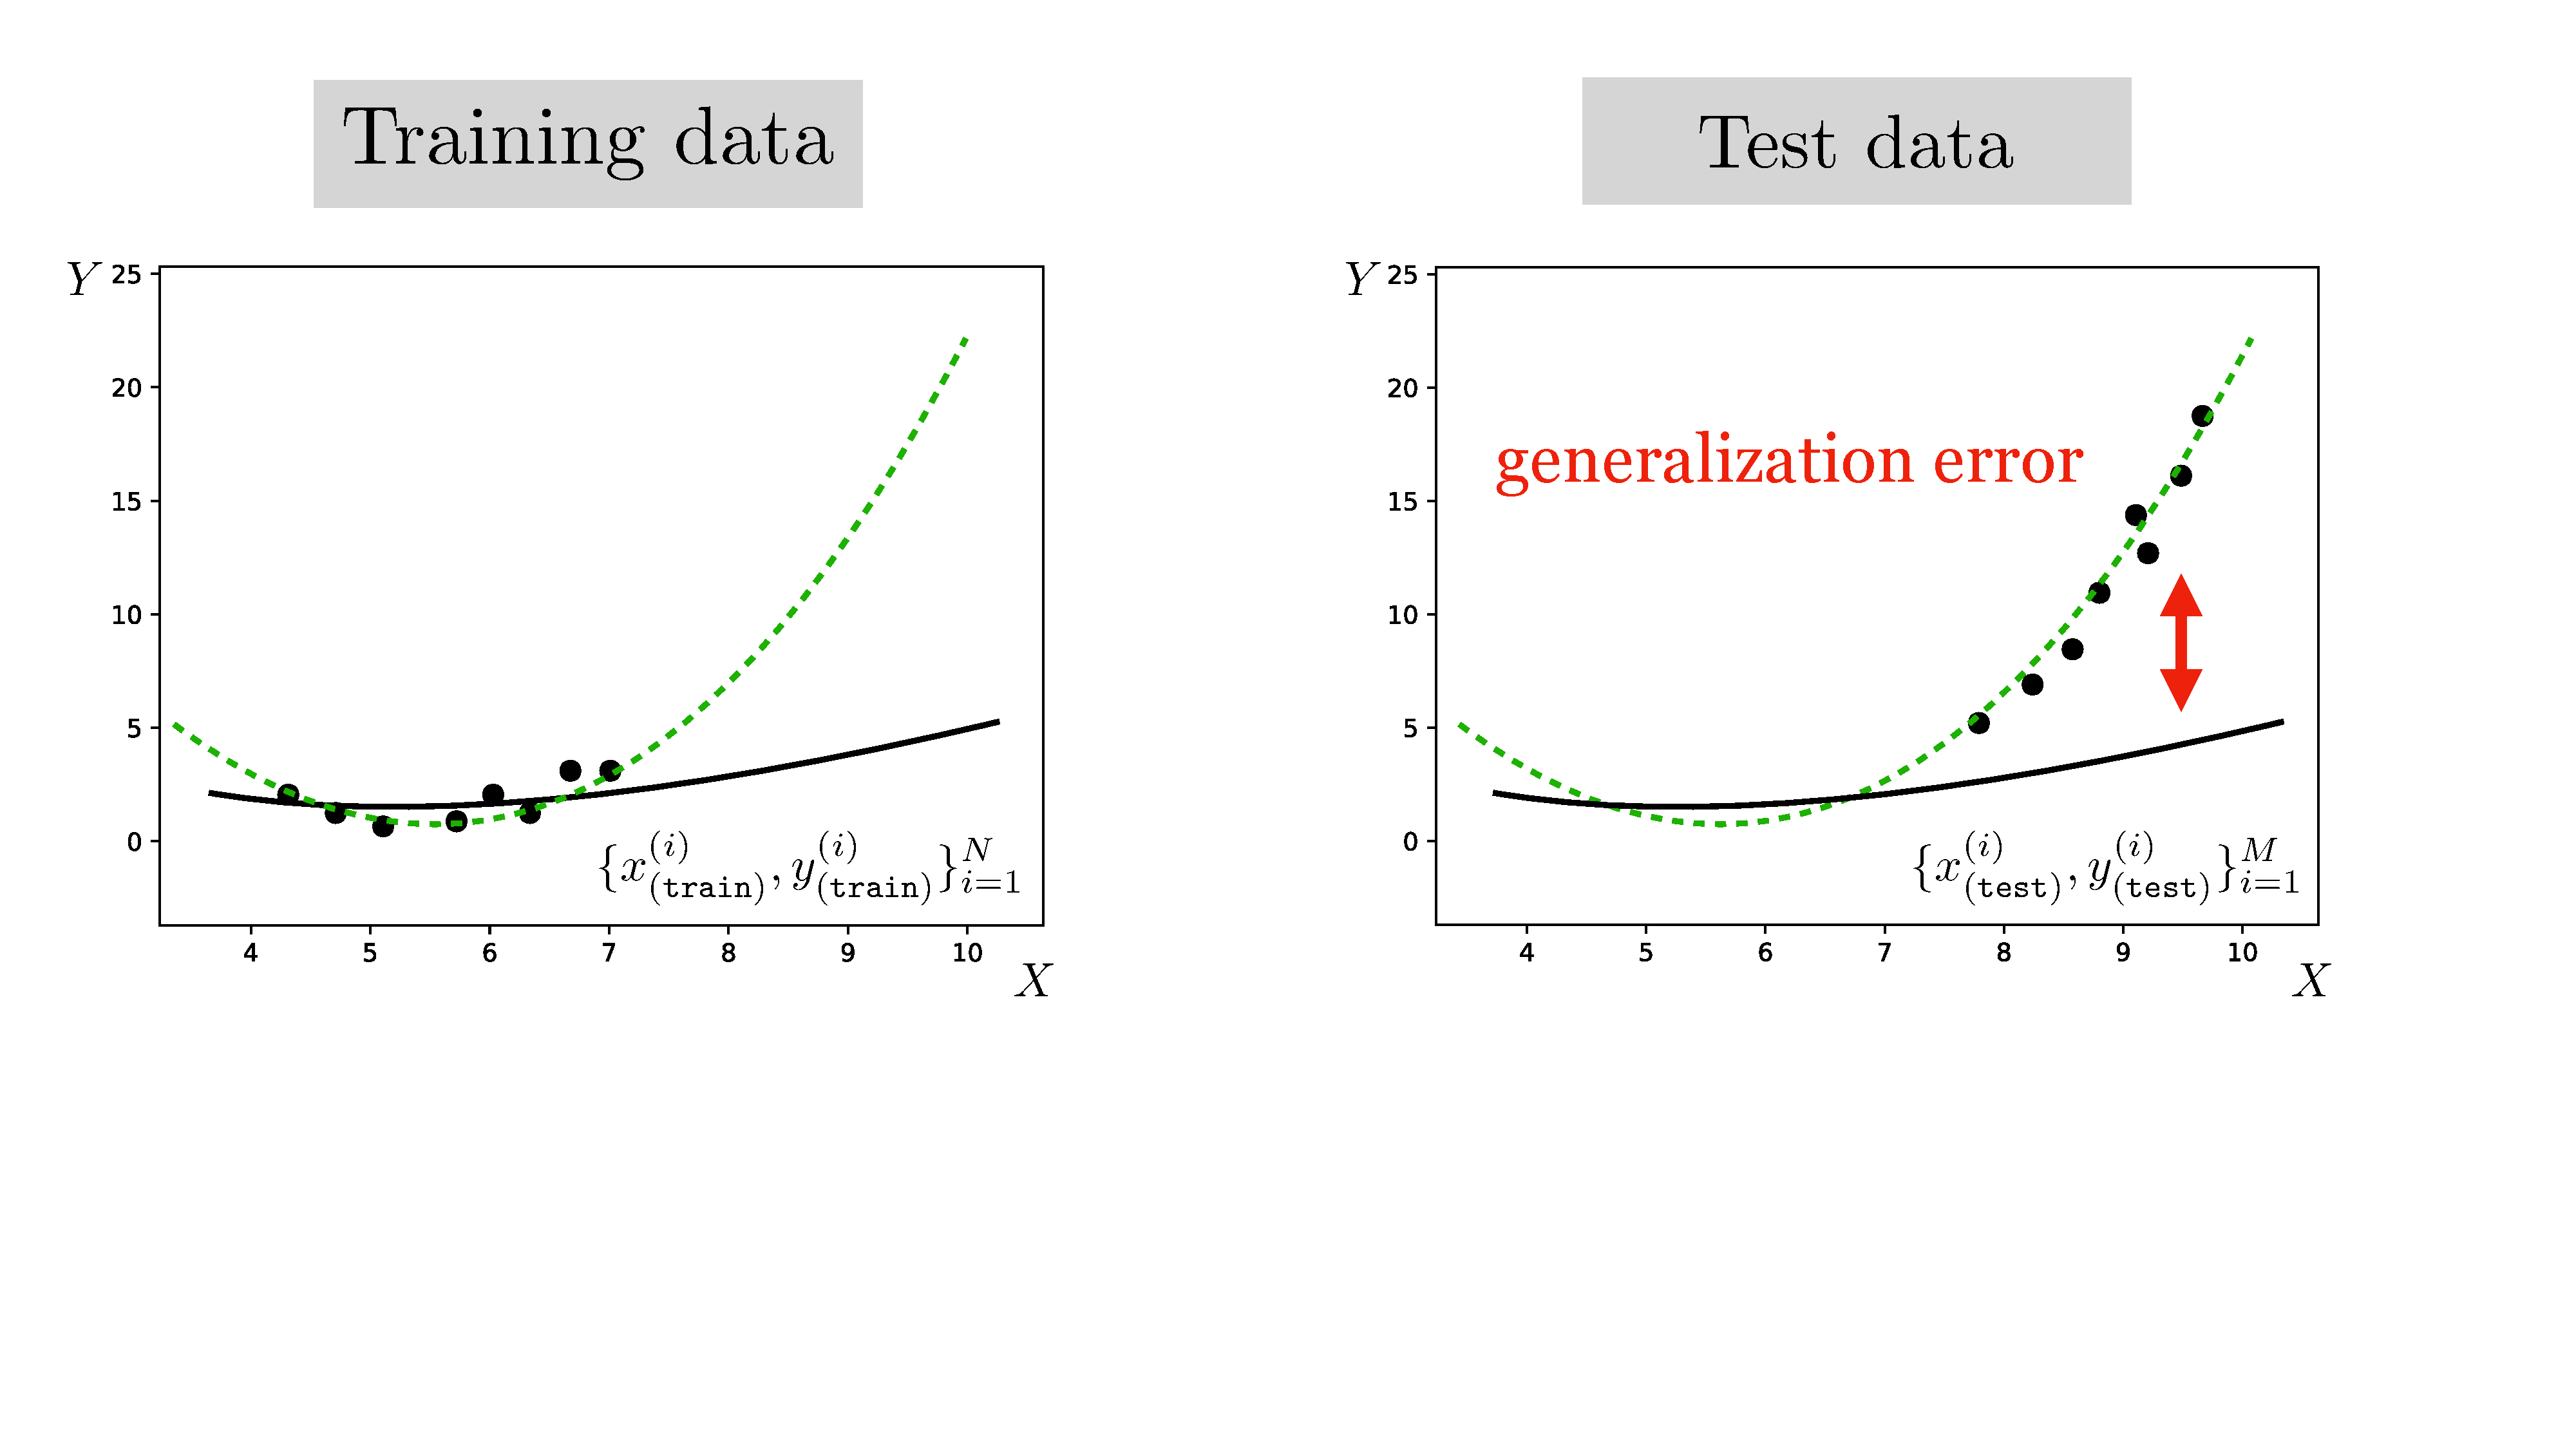
\includegraphics[width=1.0\linewidth]{./figures/bias_and_shift/regression_example.pdf}
    }
    \caption{Generalization error can be arbitrarily bad when there is distribution shift between training and test.}
    \label{fig:bias_and_shift:regression_example}
\end{figure}

The green line indicates the true data generating process, $p_{\texttt{data}}$. The training data is sampled from the flat part of the curve, whereas the test data is sampled from a different region, where the curve slopes sharply up. The solid black line is the least squares fit on the training data. It is a great fit for that part of the function but not for other parts of the data space.

The same thing is happening in the colorization example: the training data is sampled from one part of the total data space and the test data is sampled from another part. There is a \index{Domain gap}{\bf domain gap} between the training distribution and test distribution, which we indicate with the red arrows in \fig{\ref{fig:bias_and_shift:colorization_domain_gap}}.

\begin{figure}[h!]
    \centerline{
    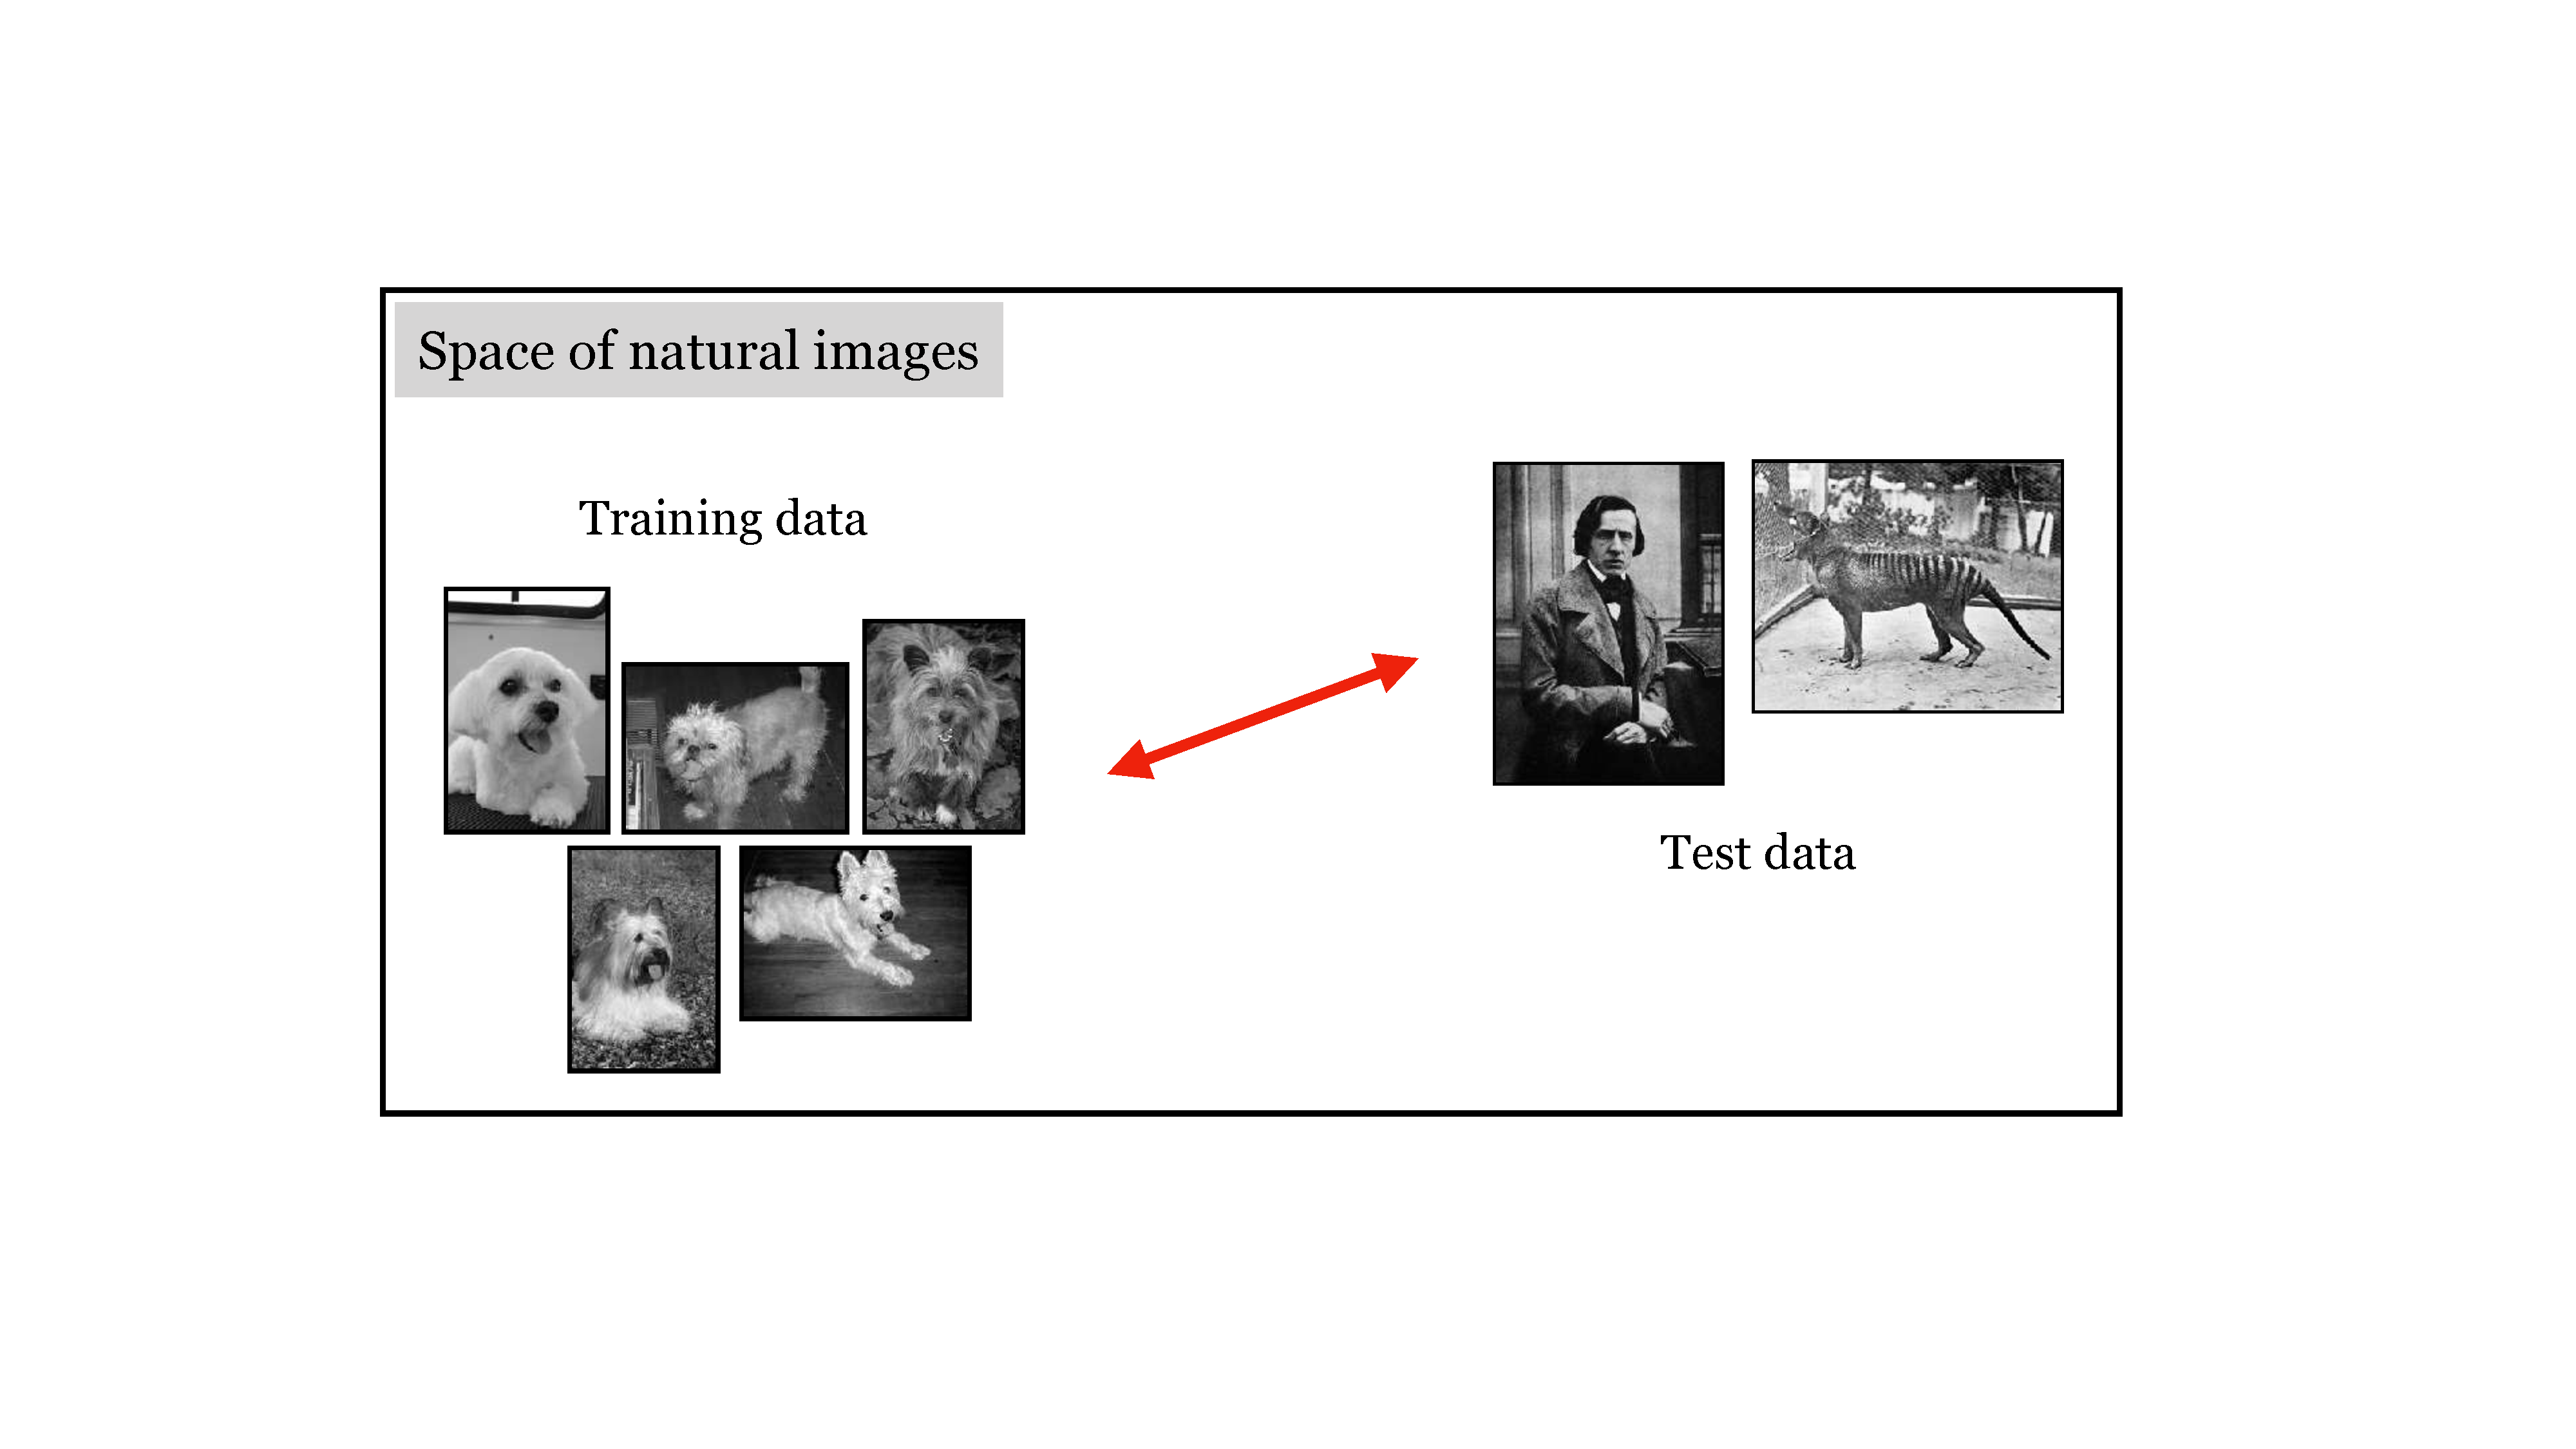
\includegraphics[width=1\linewidth]{./figures/bias_and_shift/colorization_domain_gap.pdf}
    }
    \caption{Domain gap between training data and test data in the ColorizeBot example.}
    \label{fig:bias_and_shift:colorization_domain_gap}
\end{figure}

Aside from colorizing photos on Reddit, how often do situations like this come up in the real world? \textit{All the time}. Suppose you train a weather prediction system on data from the winter months, then test it in the summer. Or train it in 2020 and test it in 2030. What would happen if there were global warming? Suppose you trained a predictive model at the beginning of the COVID-19 pandemic, based on the observed behavior at that time. What happens when people adjust their behavior? What happens if a vaccine is developed, or if a variant emerges. Financial advisors offer a disclaimer like ``past performance is no guarantee of future results.'' Why do they have to say this? In classical statistical learning theory, past performance does provide a (probabilistic) guarantee over future results. In all these cases we are confounded by a shifting data distribution. Shifting data is the rule, not the exception.

\section{A Toy Example}

Let's start by looking at toy example. In this toy example, we will consider that we have access to two datasets, each one with different data distributions. We will study the effect of training on one dataset and testing on another.
%Performance as a function of the amount of data

%Dataset value



Observations $(x,y)$ are sampled from a distribution
%\begin{equation}
%x \sim \mathcal{N}(\mu,\sigma)
%\end{equation}
where $x$ is sampled from a Gaussian and 
$y$ are noisy observations of the function $f$ applied to $x$:
\begin{align}
    x &\sim \mathcal{N}(\mu,\sigma) \\
    y & = f(x) + \beta \epsilon \\
    \epsilon &\sim \mathcal{N}(0, 1)
\end{align}
The unknown function $f$ has the form:
\begin{equation}
    f_{\theta}(x) = \theta_0 x + \theta_1 x^2 \quad\quad \triangleleft \quad\text{hypothesis space}
\end{equation}

In the first dataset, the Gaussian parameter's are $\mu_A = -1.5$, and the standard deviation is $\sigma_A = 1.5$. In the second dataset, the Gaussian has $\mu_B = 2.5$ and $\sigma_B = 0.5$. 

For each dataset we will sample two sets of examples. One set of examples will be the training set, and the other set of examples will the test set, which we will use to measure the generalization error.

Learning is done by optimizing the loss over the corresponding training set:
\begin{equation}
    J(\theta; \{x^{(i)}, y^{(i)}\}^N_{i=1}) = \frac{1}{N}\sum_i \norm{f_{\theta}(x^{(i)}) - y^{(i)}}_2^2 + \lambda \norm{\theta}_2^2 \quad\quad \triangleleft \quad\text{objective}
\end{equation}


\Fig{\ref{fig:bias_and_shift:training_test_sets}} shows training and test examples from both datasets and illustrates the effect of training on one dataset and testing on another. Each plot shows the training samples (circles), used to fit the model, and test samples (triangles) used to measure the generalization error. The diagonal plots show the training and test set corresponding to distribution A, \fig{\ref{fig:bias_and_shift:training_test_sets}}(top-left), and distribution B, \fig{\ref{fig:bias_and_shift:training_test_sets}}(bottom-right). In each case, the fitted model is shown as a dashed line.

\begin{figure}[h!]
    \centerline{
    \includegraphics[width=1\linewidth]{figures/bias_and_shift/toy_example/training_test_sets.eps}
    }
    \caption{Training and testing on different datasets. In this illustration, all datasets have 5 samples.}
    \label{fig:bias_and_shift:training_test_sets}
\end{figure}

When training and testing is done using samples from the same distribution (A to A, or B to B) the learned model (best fit) passes near the test samples and the error is small. However, when training and test are coming from different distributions, the error can be large. \Tab{\ref{table:bias_and_shift:training_test_sets}} shows the generalization error made with different combinations of training and set sets as shown in \fig{\ref{fig:bias_and_shift:training_test_sets}}. 
%[[0.17841643742260618, 0.6970794643745234], [1.9345066089885115, 0.22852186786210688]]
\begin{table}[h]
\caption{Generalization error on the test sets A and B, when training on the training samples from datasets A and B.} 
%\marginnote{{\bf Table \ref{table:bias_and_shift:training_test_sets}}: Generalization error on the test sets A and B, when training on the training samples from datasets A and B.} 
%\faketablecaption{} 
\label{table:bias_and_shift:training_test_sets}
\begin{center}
\begin{tabular}{l|l|c|c|}
\multicolumn{2}{c}{}&\multicolumn{2}{c}{Test set}\\
\cline{3-4}
\multicolumn{2}{c|}{}&A&B\\
\cline{2-4}
Training set & A & $0.18$ & $0.7$ \\
\cline{2-4}
& B & $1.93$ & $0.23$ \\
\cline{2-4}
\end{tabular}
\end{center}
\end{table}

The diagonal elements correspond to the error obtained when training on the training examples of dataset A and testing on the test examples of dataset A, and when training and testing on dataset B.  

As shown in \tab{\ref{table:bias_and_shift:training_test_sets}}, the error becomes larger for the elements off-diagonal. However, \tab{\ref{table:bias_and_shift:training_test_sets}} only gives a partial picture about what is happening because it gives the error only for dataset size equal to 5. What happens if we add more data? 

It is interesting in general to look at the performance as a function of training data. If we add more data, does performance improve when training and testing on different datasets? Or does it saturate? The answer will depend on the form of the data distributions and the hypothesis space. But we can check what happens in this toy example. 

\Fig{\ref{fig:bias_and_shift:test_as_function_of_data}} plots the generalization error (vertical axis) when evaluating on dataset A as a function of the amount of training data (horizontal axis). 


\begin{figure}[h!]
    \centerline{
    \includegraphics[width=0.6\linewidth]{figures/bias_and_shift/toy_example/test_as_function_of_data.eps}
    }
    \caption{Generalization error as a function of number of training examples. Test set is dataset A. Each curve shows the performance when training with dataset A and with dataset B (same distributions as in \fig{\ref{fig:bias_and_shift:training_test_sets}}).}
    \label{fig:bias_and_shift:test_as_function_of_data}
\end{figure}


Interestingly, both training sets (A and B) succeed in reducing the generalization error on the test set of dataset A when more training data is available. In this example, even the biased dataset B is still able to train a successful model of dataset A. However, the reduction of the error is slower than when training on dataset A. Examples from dataset B are less valuable than examples from dataset A \cite{Torralba2011}. We need approximately 10 times more examples from dataset B in order to reach a particular performance. Another way of saying this is that the value of a training example from dataset B when evaluating on dataset A is around $1/10$ of the value of a sample from A.

In this toy example, we created two datasets that had a mean shift and a standard-deviation shift. Shifts in the distributions represented by different datasets are always present. 

\section{Dataset Bias}
\index{Dataset bias}

The first thing is to notice that bias is present in all datasets. Even datasets that try to cover the same aspect of the world, they collect data with different styles and strategies that will reflect on the statistics of the dataset. In the case of image datasets for computer vision, the goal is to represent the visual world with all its complexity and diversity. Despite that there is a single visual world, different computer vision datasets offer a different, and biased, sample of that world.  

In the paper \cite{Torralba2011}, the authors propose a game that we reproduce in \fig{\ref{fig:bias_and_shift:datasetsJeopardy}}. The name of the game is {\em Name That Dataset!} 
The figure shows three random images from 12 famous computer vision datasets and the goal of the game is to match the images with each dataset name. The point of the game is to show that it is easy to recognize the {\em style} of images and to identify the dataset they belong to. If the datasets were unbiased samples of the same visual world it would be impossible to win the game, yet researchers with experience on these datasets can get around 75 percent of the matches right \cite{Torralba2011}.

\begin{figure}[h!]
    \centerline{
    \includegraphics[width=1\linewidth]{figures/bias_and_shift/datasetsJeopardy.eps}
    }
    \caption{Let's play the {\em Name That Dataset!} game. Modified from \cite{Torralba2011}. The game consists in associating each set of three images with the name of the dataset, from the list on the right, they belong to.}
    \label{fig:bias_and_shift:datasetsJeopardy}
\end{figure}

\marginnote{Answer key for \fig{\ref{fig:bias_and_shift:datasetsJeopardy}}: 1) Caltech-101, 2) UIUC, 3) MSRC, 4) TinyImages, 5) ImageNet, 6) PASCAL VOC, 7) LabelMe, 8) SUNS-09, 9) 15 Scenes, 10) Corel, 11) Caltech-256, 12) COIL-100.}[-1.15in]
One can also train a classifier to play the {\em Name That Dataset!} game automatically. We can do that by selecting a random subset of images from each dataset that we will use to train a classifier, and then we will test on new unseen images. Indeed, as shown in \cite{Torralba2011}, a classifier can play the game quite successfully. 

%Let's play a game we call {\em Name That Dataset!}  Shown in
%Figure~\ref{fig:game} are three most discriminable (to be explained
%in a moment) images from twelve popular recognition datasets.  The
%goal is to guess which images came from which dataset (go ahead, try
%it, we will wait... finished? Now check your answers
%below\footnotemark).  In theory, this should be a very difficult task
%considering that the datasets contain thousands to millions of images.
%Moreover, most of these datasets were collected with the expressed
%goal of being as varied and rich as possible, aiming to sample the
%visual world ``in the wild''.  Yet in practice, this task turns out to
%be reasonably easy for anyone who has worked in object and scene
%recognition (in our labs, most people got more than 75\% correct).


%%% Teaser
%\begin{figure}
%  \centering
%%    \includegraphics[width=\linewidth]{datasetsJeopardy2}
%    \caption{Name That Dataset: Given three images from twelve popular
%      object recognition datasets, can you match the images with the
%      dataset? (answer key below) }
%  \label{fig:game}
%\end{figure}
%%%



% https://arxiv.org/ftp/arxiv/papers/1505/1505.01257.pdf
\subsection{The Value of Training Examples}

In \tab{\ref{table:market_bias}}, each number represents the value of one training example from one dataset when used to test on another. A value of 0.25 means that you need 4 times more training examples than when using a sample derived from the same testing distribution. These results are from 2011 \cite{Torralba2011} and computer vision datasets have evolved since then.

\begin{table}[h]
\caption{``Market Value'' for a ``car'' sample across datasets. Modified from \cite{Torralba2011}.} 
%\marginnote{{\bf Table \ref{table:market_bias}}: ``Market Value'' for a ``car'' sample across datasets. Modified from \cite{Torralba2011}.} 
%\faketablecaption{} 
\label{table:market_bias}
\begin{small}
\begin{tabular}{|l|r|r|r|r|r|r|}
\hline
             & LabelMe market & PASCAL mkt. & 
ImageNet mkt. & Caltech101 mkt.  \\
\hline
%1 SUN09 is worth       & 1 SUN09 &  0.91 LabelMe &   0.72 Pascal & 
% 0.41 ImageNet & 0 Caltech  \\
1 LabelMe is worth     & 1 LabelMe &   0.26 Pascal &
 0.31 ImageNet & 0 Caltech  \\
1 Pascal is worth      & 0.50 LabelMe & 1 Pascal &
 0.88 ImageNet & 0 Caltech  \\
1 ImageNet is worth    &  0.24 LabelMe &  0.40 Pascal &
 1 ImageNet &  0 Caltech  \\
1 Caltech101 is worth  &  0.23 LabelMe &  0 Pascal &
 0.28 ImageNet & 1 Caltech  \\
\hline
%Basket of Currencies & 0.58 LabelMe &  0.48 Pascal & 
%0.58 ImageNet & 0.20 Caltech \\
%\hline
\end{tabular}
\end{small}
\end{table}

%What is the value of current datasets when used to train algorithms that will be deployed in the real world? The answer that emerges can be summarized as: ``better than nothing, but not by much''.  

\section{Sources of Bias}

There are many reasons why datasets are biased. It is important when designing a new dataset to study first the potential sources of biases associated with each data collection procedure so as to mitigate those biases as much as possible. Collecting a diverse and an unbiased dataset  usually translates to improved performance for the downstream task. We will list here some sources of bias, but this list is far from exhaustive. 

\subsection{Photographer Bias}
\index{Dataset bias!Photographer bias}

The photographer bias is probably one of the most common biases in image databases, and surprisingly difficult to get rid of it. 

In a beautiful study,  Steve Palmer et al \cite{Palmer1981}
% S. Palmer, E. Rosch, and P. Chase. Canonical perspective and the perception of objects. Attention and Performance IX, 1981.
 showed participants photographs of objects with different orientations in order to measure what orientations they preferred. For each object there were 12 different orientations. Participants had consistent preferrences for particular viewpoints for each object. Interestingly, those preferences also correlated with how easy it was to recognize each object. In another experiment from the same study, participants were shown one picture and their task was to classify the object as quickly as possible from a fixed set of twelve known possible classes. The average response time and accuracy were a measured for each of the 12$\times$12 images. The speed and accuracy are a measure of how easy is to recognize an object under a particular viewpoint. The study showed that people recognized objects better when presented in a canonical orientation. \Fig{\ref{fig:bias_and_shift:palmer_1981enhanced}} shows the preferred viewpoint for the 12 objects studied.


\begin{figure}[h!]
    \centerline{
    \includegraphics[width=1\linewidth]{figures/bias_and_shift/palmer_1981enhanced.jpg}
    }
    \caption{Cannonical viewpoints for 12 objects. Figure from \cite{Palmer1981}.}
    \label{fig:bias_and_shift:palmer_1981enhanced}
\end{figure}

The views that are recognized faster also match the viewpoints that are preferred when taking a picture of those objects \cite{Palmer1981}. Such photographer preferred viewpoint introduces biases on how objects are captured, and this bias makes the statistics of object pose in photographs different from the statistics of how objects are actually seen. The photographer bias exists for objects and scenes (composed of many objects). When taking pictures of scenes, there are biases on the preferred viewpoint, camera orientation (e.g., the horizon is usually inside the picture frame), object locations (such as the one third rule), object arrangements, positions of shadows, types of occlusions, position of the sun, time of day, weather, and so on. All of those factors are taken in consideration (consciously or not) by photographers when deciding which pictures to take.

When building a benchmark, especially when it is small, it is easy to introduce another photographer bias which is to take pictures that ``feel'' easier to recognize. This might be the right thing to do at first, when debugging a system, but, if abused, has the risk of leading us in the wrong direction when choosing which approach works best.  

These biases also apply to sequences. When filming, the user will tend to record people in certain configurations, or have the camera position in a specific orientation which respect to the main direction of the action, etc. Movie directors also use a number of techniques to capture shots that produce special viewpoint distributions. 

\subsection{Collection Bias}
\index{Dataset bias!Collection bias}

There are many potential data sources, all with different biases; Egocentric videos, internet images, vacation photographs, video captured from a moving vehicle, etc. The potential biases from each data source can be quite significant, and it's often straightforward to identify the capture technique merely by examining the images in a dataset.  

\Fig{\ref{fig:bias_and_shift:mugs}} shows the first 22 images returned by Google for the query ``mug.'' It looks far from a diverse and unbiased collection of images. As you can appreciate these pictures of mugs look very different from the visual settings in which one usually encounters mugs (inside cabinets, on top of a table, inside the dishwasher, or dirty inside the sink). Instead the images that appear in the search are taken against a flat background, mostly just white, and under a very canonical point of view. For instance, there are no views directly from above. Other biases can be a bit subtle, for example, most of the handles appear on the right side, and most of the mugs are fully visible, without any occlusions from hands or other objects, and the only two cases of occlusions from mugs occluded by another mug.


\begin{figure}[t]
    \centerline{
    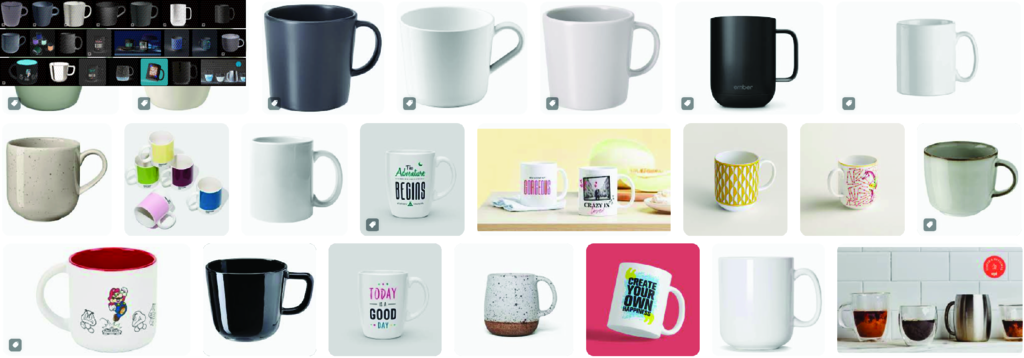
\includegraphics[width=1\linewidth]{figures/bias_and_shift/mugs.eps}
    }
    \caption{Pictures of mugs returned by a Google image search. There are many types of biases present in this small image collection.}
    \label{fig:bias_and_shift:mugs}
\end{figure}

The example of the mug, although a bit of a caricature, helps to understand some of the biases that come from the particular collection protocol used to collect images. In this case, images on the internet have a particular type of bias (at least of the ones that get returned under specific searches). 

\Fig{\ref{fig:bias_and_shift:horses}} shows images returned when looking for ``horse.'' Interestingly many of the pictures are similar to the horse canonical orientation shown in \fig{\ref{fig:bias_and_shift:palmer_1981enhanced}}.

\begin{figure}[h!]
    \centerline{
    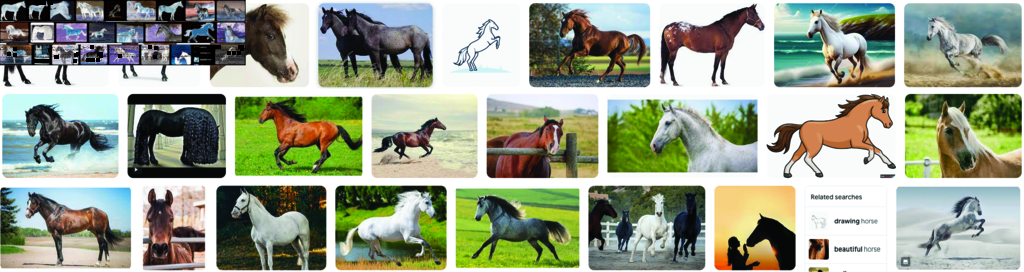
\includegraphics[width=1\linewidth]{figures/bias_and_shift/horses.eps}
    }
    \caption{Pictures of horses returned by a Google image search. There are many types of biases present in this small image collection.}
    \label{fig:bias_and_shift:horses}
\end{figure}



\subsection{Annotation Bias}
\index{Dataset bias!Annotation bias}

When annotating images, image annotators will choose which images to annotate and which labels to use. This will also correlate with viewpoint preferences and other photographer biases as those images might be easier to annotate and segment, and this has the risk of compounding with the photographer bias. 

Annotations will require making language choices and that are an important source of bias, especially social bias.

\subsection{Social Bias}
\index{Dataset bias!Social bias}

This type of bias can affect both the images and the associated labels. Social bias refers to biases associated to how groups of people  might be reflected differently in the data. Social biases can be originated by the data collection protocol or by existing social biases.  Images can be captured in certain world regions, or contain stereotypes. Labels can reflect social assumptions and biases. An example of social bias is a dataset of images and labels that associates doctors with males and nurses with females.


These types of biases, besides impacting the overall model performance, can have a negative social impact once they are deployed. It is important to be aware of those biases, and incorporate techniques to mitigate their effects. Now it is a good moment for the reader to revisit \chap{\ref{chapter:computer_vision_and_society}}. 


\subsection{Testing and Benchmark Bias}
\index{Dataset bias!Testing and benchmark bias}

One usually thinks about the biases in the training set, but biases in the test set can have an even more negative impact on the final system behavior than the training bias. The test set is what researchers and engineers use to decide which algorithm is best, or what data collection is more effective for training. However, there might be little correlation between the performance measured on the test set and the final performance of the system during deployment.

In particular, if we compare two training datasets, one biased and another less biased, by evaluating the performance of a system trained on them using a biased test dataset, we could reach the conclusion that the biased dataset is better.
\marginnote{Remember that ``bias'' is a relative term between two datasets, or between a dataset and the real world, or a desired distribution. We only have access to the real world via datasets (which inevitably are biased).}

%\section{Bias Mitigation}

\section{Adversarial Shifts}

The data shifts described previously may be disconcerting, but at least they are not malicious. Unfortunately, things can get worse. Quite often the data shift is not just random but adversarial. This may come up whenever our test setting is under the control of a competing agent, for example, someone trying to hack our system (computer security), another animal trying to eat us (evolution), or a trader trying to outperform us on the stock market (finance). Worse still, the neural nets we have seen in this book are very easy to fool by an adversary. 

\subsection{Adversarial Attacks}\label{sec:bias_and_shift:adversarial_attacks}
\index{Adversarial attacks}

This was famously demonstrated by \cite{szegedy2014intriguing}, who showed that one can add imperceptible noise to an image that fools neural net classifiers despite looking completely innocuous to a human. In fact, the noise pattern can be selected to force the network to produce any output the attacker desires. These are called {\bf adversarial attacks} because we suppose the attacker, who adds the noise, is an adversary that wants to fool or manipulate your system. The adversary can do this by simply optimizing the noise pattern to cause the network to make a particular output, while restricting the noise to be very subtle (within an small $r$-radius ball around the original image). For example, to cause an image classifier $f$ to think the cat in \fig{\ref{fig:bias_and_shift:adversarial_perturbation}} is an ostrich, the attacker could find the noise pattern via the following optimization:
\begin{align}
    \argmax_{\mathbf{\epsilon}} H(\mathbf{y}_{\texttt{ostrich}}, f(\mathbf{x} + \mathbf{\epsilon})), \quad\quad \text{subject to} \quad\quad \norm{\mathbf{\epsilon}} < r
    %\argmax_{\mathbf{r}} p(Y = \texttt{ostrich} \given \mathbf{x} + \mathbf{r}), \quad\quad \text{subject to} \quad\quad \norm{\mathbf{r}} < \epsilon
\end{align}
where $H$ is the cross-entropy loss and $\mathbf{y}_{\texttt{ostrich}}$ is a one-hot code for the ostrich class.

\begin{figure}[t]
    \centerline{
    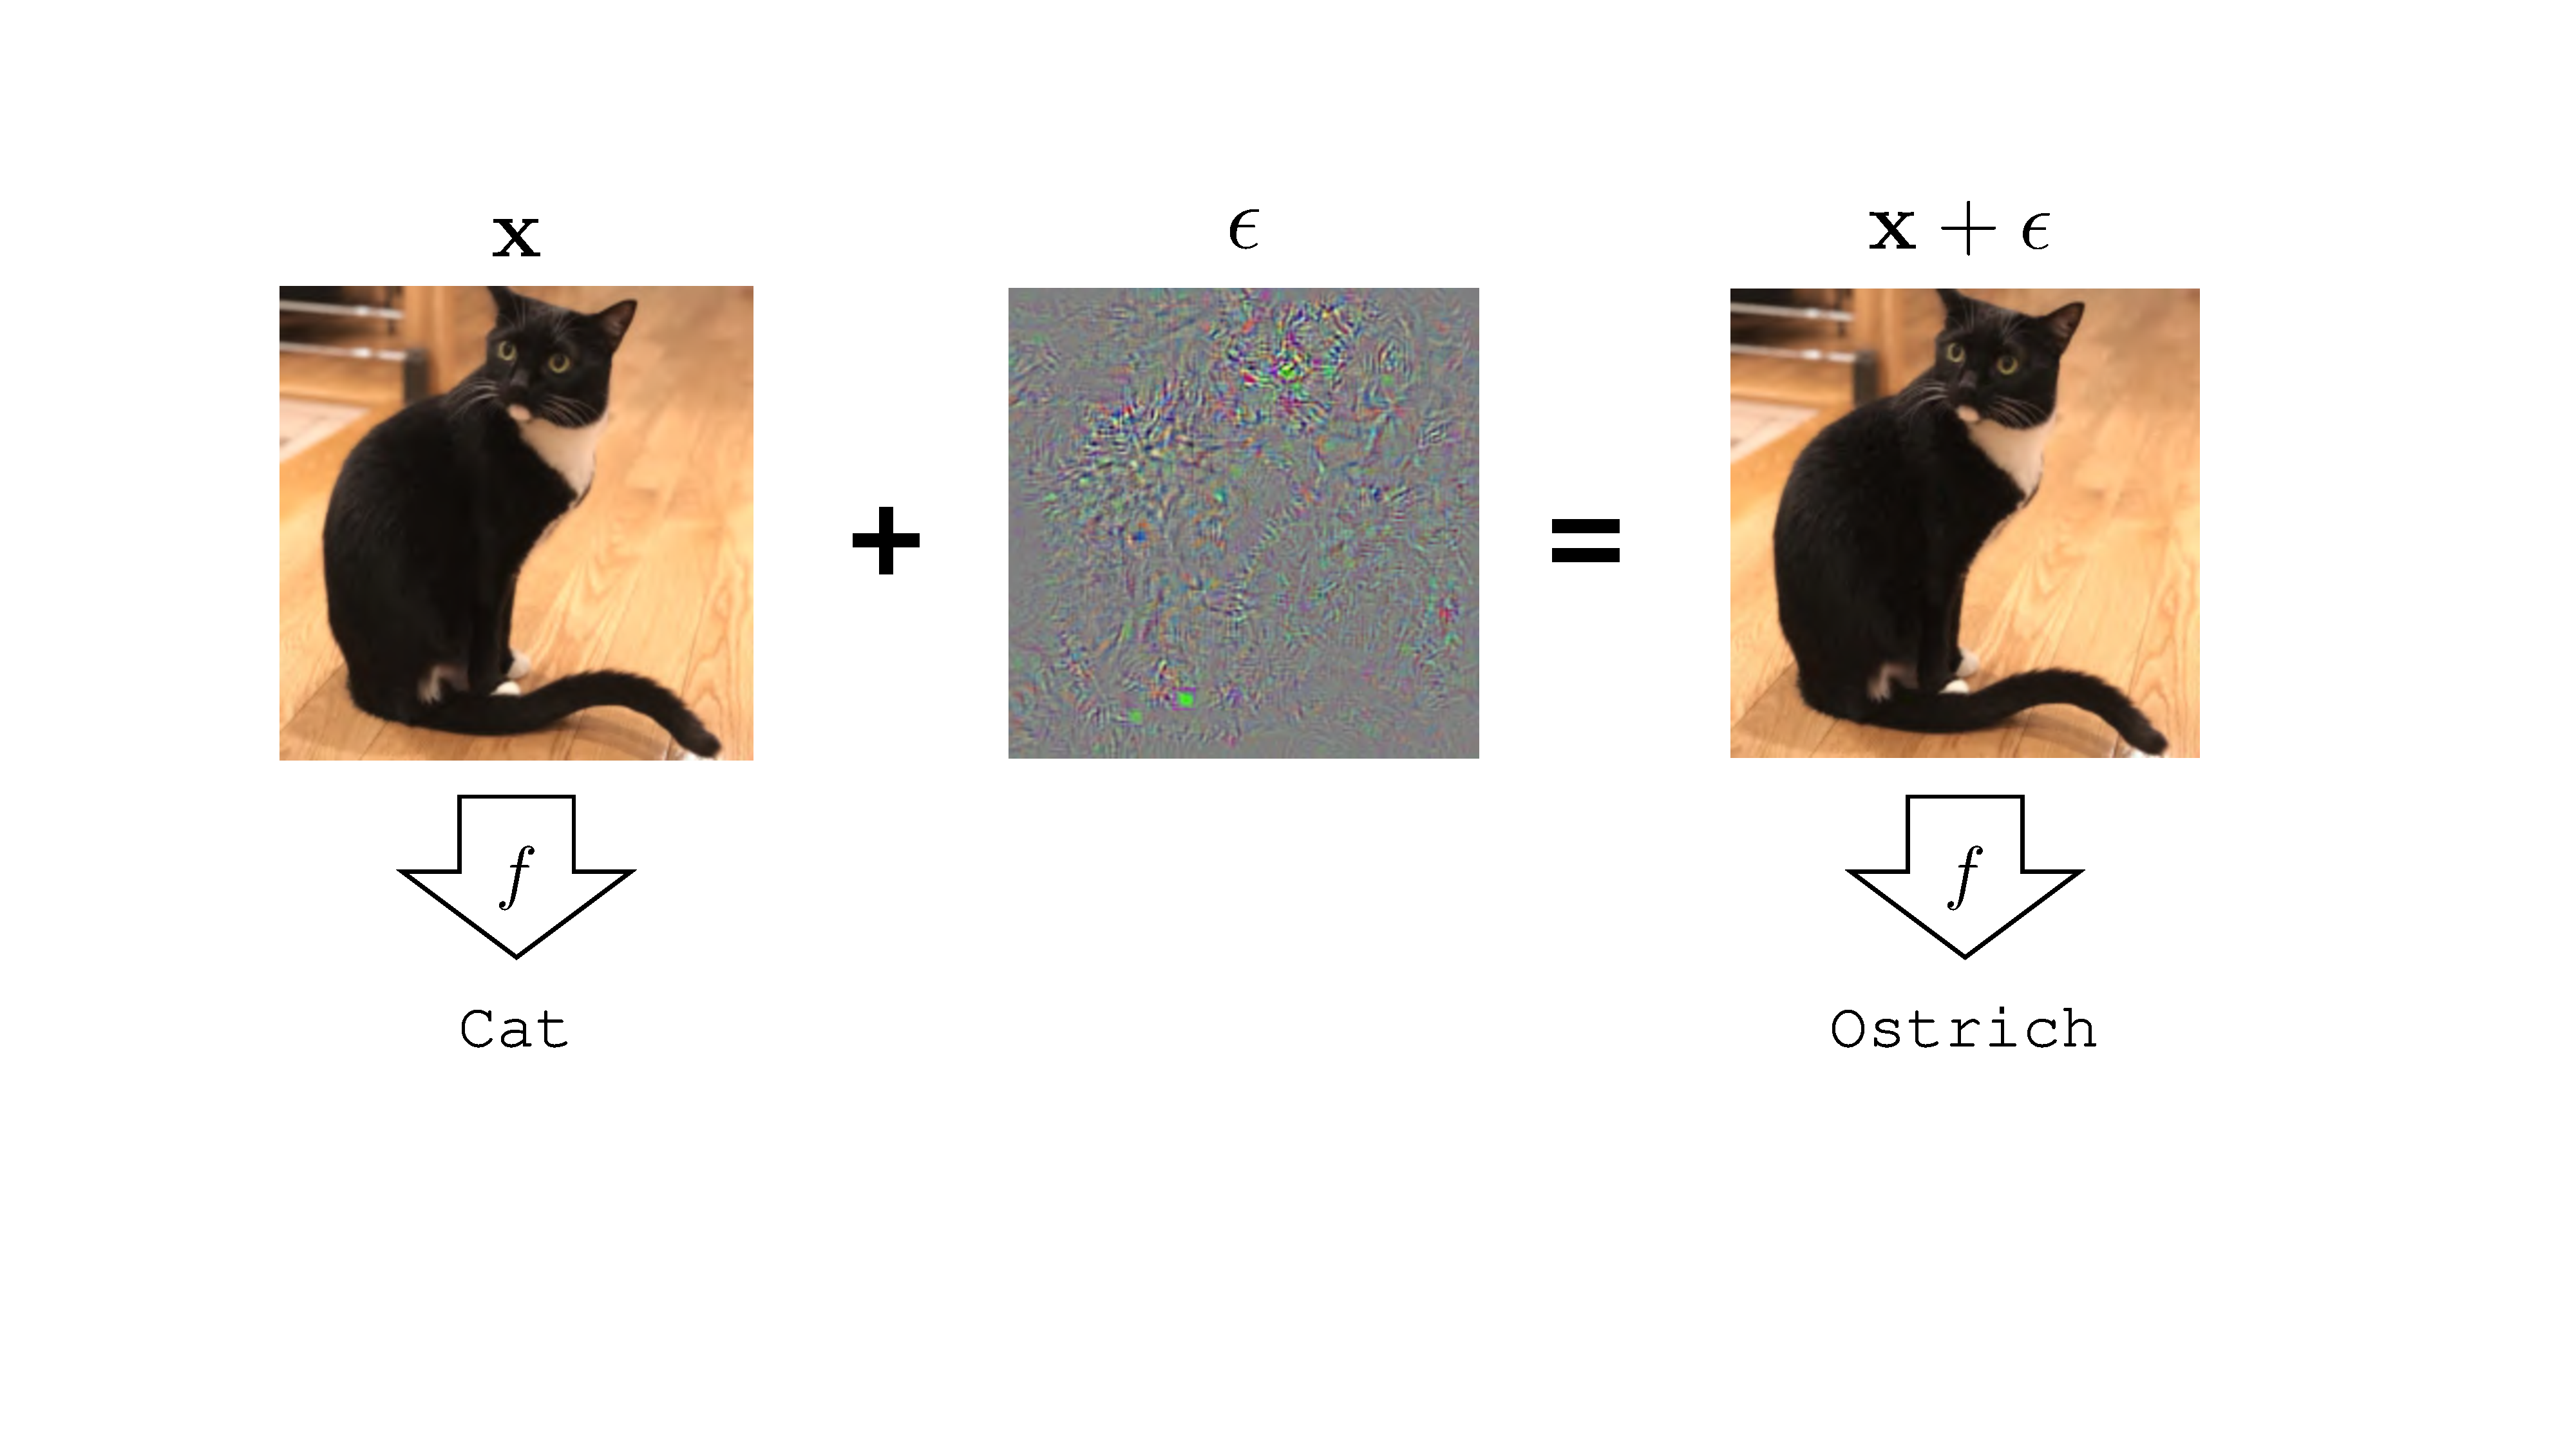
\includegraphics[width=0.8\linewidth]{./figures/bias_and_shift/adversarial_perturbation_3.pdf}
    }
    \caption{An adversarial attack that adds subtle changes to the cat photo to make a neural net classify it instead as an ostrich. The noise image color values are scaled 20x for visualization.}
    \label{fig:bias_and_shift:adversarial_perturbation}
\end{figure}

This type of attack required that the attacker has access to your system (the neural net $f$) so that they can optimize the noise pattern $\mathbf{\epsilon}$ to fool the system. Unfortunately, if you want to deploy your system to the public, then you have to give people access to it and that makes it vulnerable to attack.

In \chap{\ref{chapter:neural_nets}} we described a simple neural network for line classification and showed how, by accessing the architecture and the learned filters, we could manually design input examples that would get wrongly classified. Similarly, in \chap{\ref{chap:downsampling_and_upsampling}} we showed how aliasing could also create vulnerabilities in a network. For large systems, adversarial attacks are not manually designed, instead they are the result of an optimization procedure that optimizes the noise pattern $\mathbf{\epsilon}$ so that it has a small amplitude (i.e., it is imperceptible) and makes the system fail with high confidence. 

\subsection{Defenses}

Adversarial analysis is worst case analysis. Remember that we typically train our systems to minimize empirical risk, defined as the \textit{mean} error over the training data. Because we only focus on the mean, the \textit{worst case} might be arbitrarily bad. Alternative approaches try to minimize worst-case error, and this can result in systems that are more \index{Adversarial robustness}{\bf adversarially robust}.
In \chap{\ref{chapter:data_augmentation}} we will discuss how {\bf adversarial training} can be used to increase the robustness of the models to adversarial attacks. 

%It's possible to modify our objective to minimize worst case performance, under adversarial data, and in fact many models do so, including some we have seen like GANs and curiosity.

%In the next chapter, we will see some ways of dealing with domain shift using the following strategy: if things change, adapt.



% How to deal?
% I. train time
% 1. collect better data
% 2. add data augmentation
% 3. add architectural invariances
% 4. train for robustness
% II. test time
% 1. adapt




%Now for a example from vision. We will look at a case study on the paper ``Colorful Image Colorization"~\cite{zhang2016colorful}, which one of the authors of this book co-authored in 2016.




%Simpson's paradox

%Dataset bias
%Domain shift
%Adversarial examples


\section{Concluding Remarks}

One way to reduce the issues of dataset bias and shift is to implement a rigorous data collection procedure that tries to minimize the biases present in the data. Although it is possible to prevent (or reduce) certain forms of bias, others will remain challenging because it is hard to collect the necessary data or because we are not aware of it. In many cases, deployment will be done in specific settings that might be unknown a priori. Therefore, bias is here to stay and it is important to study forms to reduce its methods in the system performance.  

There are two general ways of dealing with dataset bias and shift. The first is called domain randomization, or data augmentation. The second is called transfer learning, or model adaptation. The next two chapters are about these options.
